\chapter{Implementation}
\label{chapter:methods}

\section{Qt Developer Days 2011 Conference Schedule Application}
\label{section:devdays}

The Qt Developer
Days\footnote{\url{http://qt.nokia.com/qtdevdays2011/}} is a
conference for developers using the Qt cross-platform application and
user interface framework\footnote{\url{http://qt.nokia.com/}}. We
created a mobile web application with contextual and personalized
session information and daily schedule for the conference.

\subsection{Requirements}

The target group for the conference application was mobile developers
attending the Qt Developer Days conference. Therefore, we could expect
a good technical knowledge and high-end mobile devices from the target
audience.

A native version of the application was built for devices with Qt
support, and the HTML5 application was for all other devices. The main
target devices were iPhone, Android devices, Windows Phone 7 devices,
and iPad. In addition to these, the application was tested on devices
running Symbian and Meego, as well as desktop browsers.

The conference was expected to have some thousands of attendees, of
which a few hundred was expected to use the web application. In
conferences of this size, network connectivity and reliability is
often a problem. Also, mobile networks other than the \abbr{WiFi}
network supplied by the conference might be too expensive for users
that come from other countries. This is why offline support was
needed.

The client wanted high interactivity and personalization in the
application. Users could save interesting sessions to their favorites,
which were shown in the home view of the application. The home view
was expected to be contextual in taking into account the current time
and showing the ongoing sessions and the remaining time for them, as
well as the time left for later favorite sessions to start. Current
time was also expected to be indicated in the agenda view, where a red
line was to be drawn to the current time for easily visualizing the
ongoing sessions. By default, the agenda view should show the ongoing
day of the conference if possible.

The user interface was required to use the touch input interactions
for panning and zooming the floor maps of the conference venue. Also,
the client wanted a touchable star rating widget on the feedback form
for easy and visual session rating on touch screens.

\subsection{Application Architecture}

\begin{figure}[ht]
  \begin{center}
    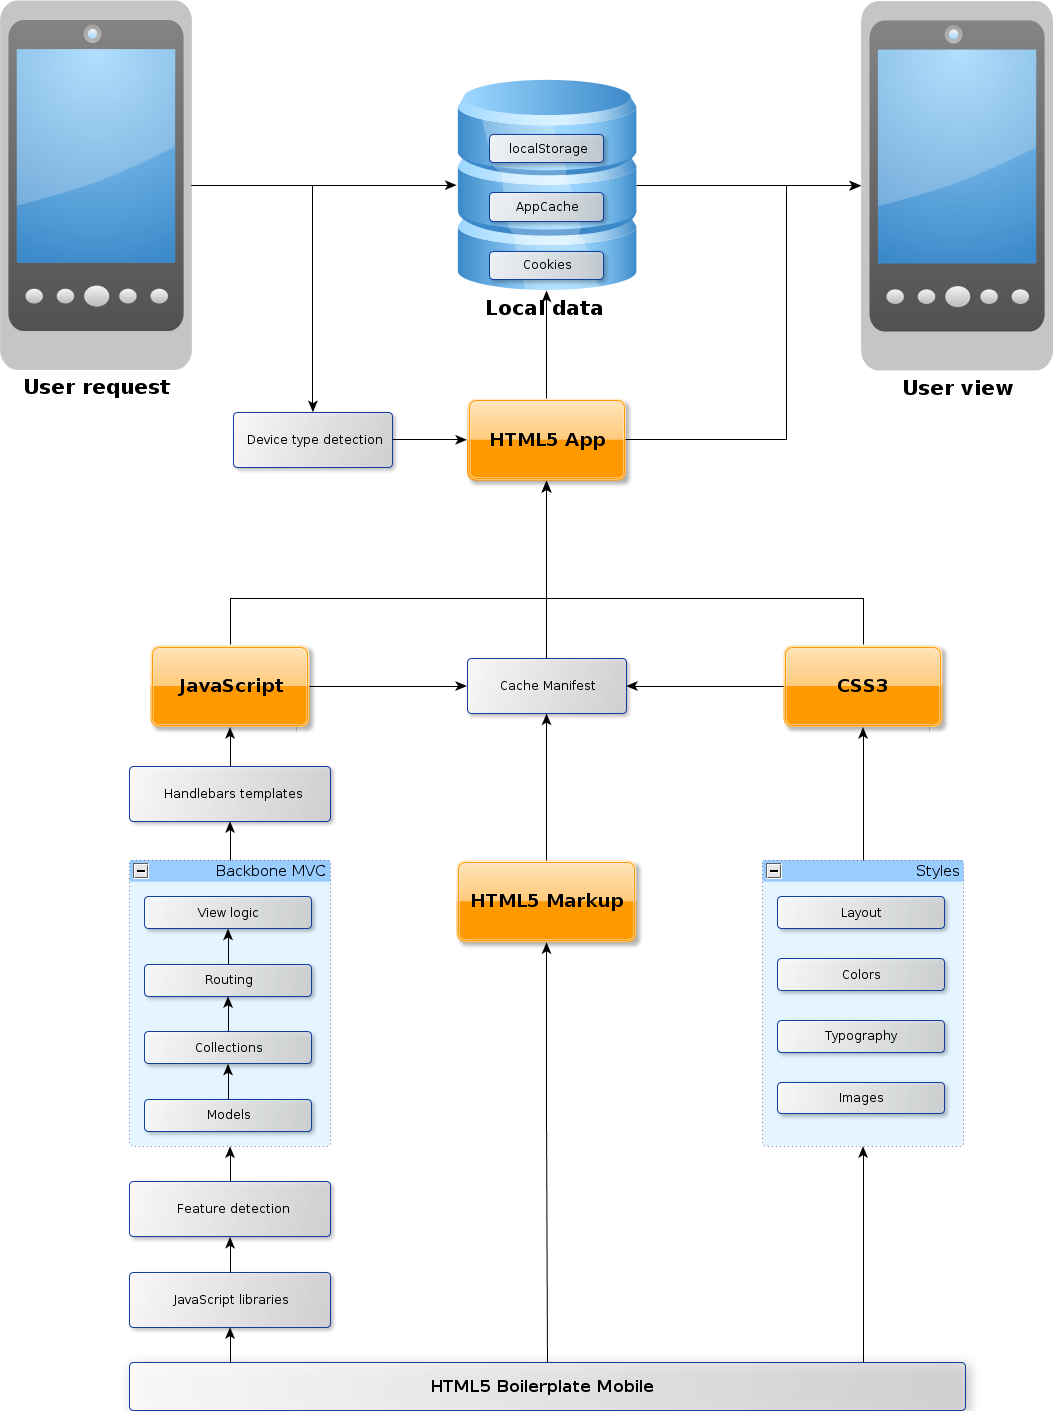
\includegraphics[width=\textwidth]{images/devdays.png}
    \caption{Conference schedule application architecture.}
    \label{figure:devdays.png}
  \end{center}
\end{figure}

The conference
schedule\footnote{\url{http://m.qtdevdays2011.qt.nokia.com/}} is a
single-page application (see
Section~\ref{section:single-page-applications}) with a lightweight
backend written in Python using the Django Web
Framework\footnote{\url{https://www.djangoproject.com/}}.

The backend provides the static assets (JavaScript, \abbr{CSS},
images, etc.) and an \abbr{API} for persisting session feedback to a
MySQL\footnote{\url{http://www.mysql.com/}} relational database. It
also generates the HTML5 AppCache (see Section~\ref{section:appcache})
offline cache manifest file based on the categorized device type.

The frontend is a JavaScript application written using the
Backbone\footnote{\url{http://backbonejs.org/}} \abbr{MVC} framework
(see Section~\ref{section:js-mvc}). Other used JavaScript libraries
include Underscore\footnote{\url{http://underscorejs.org/}} for data
manipulation, jQuery\footnote{\url{http://jquery.com/}} for \abbr{DOM}
API abstraction, Handlebars\footnote{\url{http://handlebarsjs.com/}}
for templating, and
Modernizr\footnote{\url{http://www.modernizr.com/}} for feature
detection. The HTML5 Mobile
Boilerplate\footnote{\url{http://html5boilerplate.com/mobile}} was
used as an initial markup structure for the application. The
architecture of is shown in Figure~\ref{figure:devdays.png}. Wireless
networks can be unreliable in conference settings, so offline support
was also added using several different JavaScript techniques and HTML5
APIs.

The application was designed for touch screens on various platforms
and screen sizes. The layout adjusts to the available space and
provides rich interactive components. Integration to social networking
services was also added as an additional functionality.

\fixme{add screenshots on different devices (at least phone and tablet}

\section{JSONCache JavaScript Library}
\label{section:jsoncache}

JSONCache is a lightweight JavaScript library for fetching \abbr{JSON}
data in unreliable networks. The library was designed especially to
handle unreliable mobile networks with connection problems and short
interruptions. The goal is to avoid networking as long as possible and
failing gracefully if the network connection is not stable.

JSONCache provides two main functionalities: data caching and
attempting to fetch the data multiple times.

The caching layer uses the client side localStorage (see
Section~\ref{section:datastorage}) cache of \abbr{HTML5}. Data
requests can be done using the JSONCache \abbr{API} which always
checks the local cache first before opening any network
connections. If the data is already in the cache, the cached data is
checked for validity and if the data has not been expired, it is
returned immediately. If the data is not in the cache or it has been
expired, a new network request is made and the received data is cached
and returned. The expiration time of a data item can be configured in
the library settings.

JSONCache also tries to fetch the data multiple times to handle small
interruptions in network connections.  For example, when a user leaves
his or her work place and uses a web application, the mobile device
changes from the workplace \abbr{WiFi} network to the \abbr{3G}
network, there is a short interruption in the connection, and any
ongoing network requests are affected.

If a data fetch fails, a new fetch is issued after a timeout (defined
in the configuration). On subsequent attempts the timeout is
increased, and after a defined number of attempts the fetch error is
issued.

Figure~\ref{figure:jsoncache-demo.png} shows an interactive demo of
the JSONCache library. The
demo\footnote{\url{http://kpuputti.github.com/JSONCache/demo/index.html}}
simulates the caching and fetching functionality of the library by
simulating an unreliable network based on the configuration.

\begin{figure}[ht]
  \begin{center}
    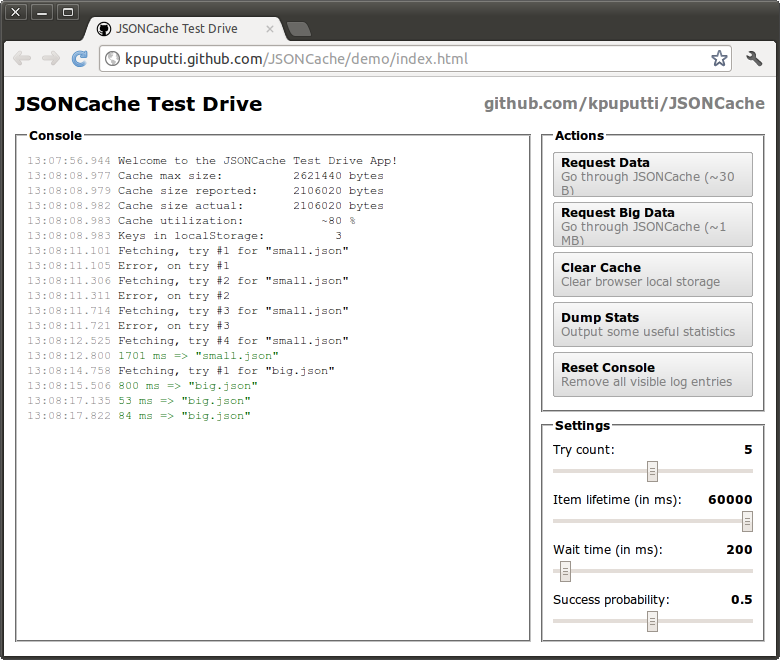
\includegraphics[width=\textwidth]{images/jsoncache-demo.png}
    \caption{Interactive JSONCache demo.}
    \label{figure:jsoncache-demo.png}
  \end{center}
\end{figure}
